\documentclass[]{IEEEtran}

\title{Modellazione e Sintesi di un Moltiplicatore Floating-point Single Precision}
\author{Enrico Sgarbanti - VR446095}

\usepackage{graphicx}
\usepackage[italian]{babel}
\usepackage[utf8]{inputenc}

\begin{document}
\maketitle

\begin{abstract}
    Gli obiettivi di questo progetto sono:
    \begin{itemize}
        \item Sviluppare in VHDL, Verilog e SystemC un moltiplicatore in virgola mobile a precisione singola e un componente che permetta di eseguire due moltiplicazioni in contemporanea.
        \item Creare i testbench per verificare la corretteza dei componenti.
        \item Sintetizzare i componenti scritti in VHDL e Verilog.
        \item Eseguire High-Level-Synthesis del moltiplicatore a precisione singola.
    \end{itemize}
\end{abstract}


\section{Introduzione}
Il sistema è composto da un modulo top-level chiamato ``double\_multiplier'' il quale esegue la moltiplicazione di due operandi dati in input nello stesso ciclo di clock in cui ready viene posto a 1, e i due opereandi passati al ciclo di clock successivo

Nell'introduzione viene descritto in maniera astratta quello che poi viene dettagliato nel seguito del report. Una buona scaletta per l'introduzione può essere la seguente:
\begin{itemize}
\item Descrizione ad alto livello delle principali caratteristiche del sistema che si vuole modellare.
\item Descrizione delle motivazioni principali per l'utilizzo delle tecnologie descritte nel corso. Qual è il problema che si vuole risolvere?
\item Descrizione dei passi utilizzati per arrivare all'implementazione finale. Descrivere la motivazione di ciascun passo. La descrizione dei passi dovrebbe formare la descrizione del flusso di lavoro svolto per completare l'assignment.
\item Rapidissima descrizione dei risultati principali.
\end{itemize}

L'introduzione non dovrebbe andare oltre la metà della seconda colonna (nel caso a due colonne), o la prima pagina (nel caso a colonna singola): bisogna cercare di essere concisi (e chiari). Alla fine, l'introduzione è solo ``chiacchiere'': deve semplicemente rendere chiari quali sono gli obiettivi del lavoro (\emph{e nel caso del corso, deve far capire a me che avete gli obiettivi chiari in testa}). Consiglio: l'introduzione (e spesso l'abstract) è l'ultima parte che viene completata.

\section{Background}
In questo progetto sono stati utilizzati diversi linguaggi per descrivere hardware a livello RT ovvero Verilog, VHDL e SystemC. 
- descrivere cos'è un floating-point
- descrivere la moltiplicazione
- arrotondamento numero binario
- handshake

Il background dovrebbe contenere una descrizione, abbastanza breve, dei concetti principali che vengono utilizzati nel lavoro. Ad esempio, può contenere una breve descrizione delle caratteristiche principali degli HDL , e delle sue estensioni. Una colonna dovrebbe bastare.

In questa sessione saranno citati anche lavori dello stato dell'arte. Ad esempio, si può usare~\cite{SystemC} per citare SystemC. \textbf{I riferimenti bibliografici vanno inseriti ogni volta in cui si va a citare qualcosa contenuto in un documento.}

Questa sessione non deve ripetere quanto detto a lezione, ma dare un overview dei concetti principali utilizzati durante lo svolgimento dell'elaborato.


\section{Metodologia applicata}
Attuando un approccio bottom-up, prima si definiscono i componenti principali cioè il {\it moltiplicatore} e il {\it doppio moltiplicatore}, descrivoli con EFSM. Dopodichè si passa all'implementazione a livello RTL in vhdl e verilog di queste e alla creazione di un piccolo testbench. A questo punto si traduce il tutto in systemC dove con la potenza del C++ si crea un testbench più complesso. Infine si procede alla sintesi e alla sintesi ad alto livello per poi confrontare i vari risultati.
I vincoli sono:
\begin{itemize}
\item Un moltiplicatore dovrà essere scritto in verilog e uno in VHDL.
\item Gli operandi e il risultato devono essere a 32 bit.
\item Deve poter essere sintetizzabile sulla FPGA  ``xc7z020clg400-1''. Essa ha disposizione solo 125 porte. Per rispettare il limite viene utilizzata la stessa porta per il risultato e due porte per gli operandi. Quindi al primo ciclo di clock con ready uguale 1, verranno trasmessi i primi due operandi e al ciclo successivo gli altri due. Dopodichè si aspetterà il complementanto delle moltiplicazioni e verrà trasmesso il primo risultato quando done varrà 1, e il ciclo di clock successivo l'altro.
\end{itemize}

\subsection{Modellazione della EFSM del moltiplicatore {\it Figure \ref{fig:EFSM1}}}
I segnali utilizzati per la comunicazione sono:
\begin{itemize}
\item \textit{\textbf{rst:}} (1 bit) per riportare il sistema allo stato iniziale .
\item {\it\bf ready:} (1 bit) per permettere al sistema di uscire dallo stato iniziale .
\item \textbf{\textit{f}} {\it {\bf norm\_again:} } (1 bit) per indicare se fare un'altra normalizzazione del numero intermedio .
\item {\it\bf res\_type:} (2 bit) per indicare se il risultato vale 0, NAN o \(\infty\) e quindi andare direttamente allo stato finale oppure se è un numero (il caso denormalizzato viene gestito come se fosse normalizzato) e quindi proseguire nell'elaborazione.
\end{itemize}

Sono inoltre necessari 14 stati:
\begin{itemize}
\item {\it\bf ST\_START:} in cui si pone {\it done} e {\it norm\_again} uguali a 0 e si ottengono le informazioni di segno, esponente e mantissa dei due operandi. In esso si rimane finchè {\it ready} vale 0 altrimensi si passa a {\it ST\_EVAL1}.
\item {\it\bf ST\_EVAL1:} e {\it ST\_EVAL2} in cui viene valutato il tipo dei due operandi fra {\it T\_ZER, T\_INF, T\_NAN e T\_NUM}
\item {\it\bf ST\_EVAL3:} in cui si ricava il tipo del risultato in base al tipo degli operandi.
\item {\it\bf ST\_CHECK1:} dove si passa a {\it ST\_FINISH} se {\it res\_type} è diverso da {\it T\_NUM}.
\item {\it\bf ST\_ELAB:} in cui si sommano i due esponenti e si sottrae 127 perchè entrambi, per lo standard, sono incrementati di 127 (\((esp+127) = (esp1+127)+(esp127) - 127\)). Per compiere la somma è necessario usare una variabile ``esp\_tmp'' 10 bit altrimenti si andrebbe in overflow per valori invece leciti che ritornerebbero validi dopo la sottrazione di 127. Inoltre viene eseguita anche la moltiplicazione delle due mantisse, che essendo a 23 bit più un bit che vale sempre 1, necessita di una variabile ``mant\_tmp'' di 48 bit 
\item {\it\bf ST\_UNDERF:} in cui si verifica se l'esponente del risultato è in uno stato di underflow, ovvero guardando se il bit {\it esp\_tmp[9]}, che nel complemento a 2 indica il segno, è 1. Infatti i valori disponibili per l'esponente vanno da 0 a 255.
\item {\it\bf ST\_CHECK2} dove si passa a {\it ST\_FINISH} se {\it res\_type} è diverso da {\it T\_NUM}, perchè diventato {\it T\_ZER} per l'underflow.
\item {\it\bf ST\_NORM1:} in cui si compie la normalizzazione della mantissa che deve sempre essere della forma {\it 1.valori}. Essendo la virgola posta tra il 46esimo bit e il 45esimo, si verificano due casi: Se il 47esimo bit vale 1 bisogna incrementare l'esponente, altrimenti il valore è già corretto, ma viene effettuato uno shift a sinistra per trattare allo stesso modo i due casi durante l'arrotondamento.
\item {\it\bf ST\_ROUND:} in cui si effettua l'eventuale arrotondamento dovuto al fatto che il valore della mantissa è attualmente a 48 bit, ma bisogna portarlo a 24 bit. L'arrotondamento è fatto per eccesso, quindi si incrementerà {\it mant\_tmp[47:24]} solo se {\it mant\_tmp[23:00]} sarà \( \geq \) a ``01..1''. L'arrotondamento effettivò verrà fatto nello stato {\it ST\_NORM2}, qui ci si limita a porre {\it norm\_again} uguale a 1 per poterci andare.
\item \textit{\textbf{ST\_CHECK3:}} dove si passa allo stato \textit{ST\_NORM2} se \(\textit{norm} = 1\) oppure allo stato \textit{ST\_OVERF} se \(\textit{norm} = 0\).
\item \textit{\textbf{ST\_NORM2:}} in cui si effettua il vero arrotondamento della mantassina. Bisogna tenere conto del caso in cui sia della forma ``1..1'' e che quindi con l'incremento vada a ``0..0'' e  venga incrementato l'esponente.
\item {\it\bf ST\_OVERF:} in cui si verifica se l'esponente del risultato è in uno stato di overflow, ovvero guardando se il bit {\it esp\_tmp[8]} vale 1 ovvero se corrisponde ad un valore maggiore di 255.
\item {\it\bf ST\_FINISH:} in cui si pone {\it done} uguale 1, si ricava {\it res[31]}, ovvero il segno del risultato facendo lo XOR fra i segni degli operandi, e in base al valore di {\it res\_type} si ottiene il resto. Dopodichè si torna allo stato inziale
\end{itemize}


\subsection{Modellazione della EFSM del doppio moltiplicatore ({\it Figure \ref{fig:EFSM2}})}
I segnali utilizzati per la comunicazione sono:
\begin{itemize}
\item {\it\bf rst:} (1 bit) per riportare il sistema allo stato iniziale .
\item {\it\bf ready:} (1 bit) per permettere al sistema di uscire dallo stato iniziale .
\item {\it\bf done1:} (1 bit) che indica quando il valore attuale di ``res1'' è il risultato della moltiplicazione.
\item {\it\bf done2:} (1 bit) che indica quando il valore attuale di ``res2'' è il risultato della moltiplicazione.
\end{itemize}

Sono inoltre necessari 8 stati:

\begin{itemize}
\item {\it\bf ST\_START:} in cui si pone {\it done}, {\it ready1} e {\it ready2}uguali a 0 e si inizializzano {\it op1\_tmp1} e {\it op2\_tmp1} rispettivamenete con i valori di {\it op1} e {\it op2} i quali serviranno per il primo moltiplicatore. In esso si rimane finchè {\it ready} vale 0 altrimensi si passa a {\it ST\_RUN1}.
\item {\it\bf ST\_RUN1:} in cui si pone {\it ready1} uguale a 1, attivando quindi il primo moltiplicatore, e si inizializzano {\it op1\_tmp2} e {\it op2\_tmp2} rispettivamenete con i valori di {\it op1} e {\it op2} i quali serviranno per il secondo moltiplicatore.
\item {\it\bf ST\_RUN2:} in cui si pone {\it ready1} uguale a 0 e {\it ready2} uguale a 1, attivando quindi il secondo moltiplicatore
\item {\it\bf ST\_WAIT:} in cui si pone {\it ready2} uguale a 0 e si aspetta che {\it done1} o {\it done2} diventino 1.
\item {\it\bf ST\_WAIT1:} si arriva in questo stato se {\it done2} vale 1, cioè se il secondo moltiplicatore ha finito e si resta qui finchè non finisce anche il primo.
\item {\it\bf ST\_WAIT2:} si arriva in questo stato se {\it done1} vale 1, cioè se il primo moltiplicatore ha finito e si resta qui finchè non finisce anche il secondo.
\item {\it\bf ST\_RET1:} si arriva in questo stato quando entrambi i moltiplicatore hanno finito. Qui si pone {\it done} uguale a 1 e {\it res} uguale al risultato del primo moltiplicatore cioè {\it res1}.
\item {\it\bf ST\_RET2:} ora si pone {\it res} uguale al risultato del secondo moltiplicatore cioè {\it res2} e si ritorna allo stato iniziale.
\end{itemize}


\subsection{Implementazione RTL}
L'intefaccia del {\it double\_multiplier} è formata dai segnali di input: {\it clk, rst, ready, op1, op2}; E i segnali di output {\it res, done}. \\
L'intefaccia del {\it multiplier} è formata anch'essa dai segnali di input: {\it clk, rst, ready, op1, op2}; E i segnali di output {\it res, done}, dove:
\begin{itemize}
\item {\it clk, rst} sono collegati ai segnali analoghi del {\it double\_multiplier}.
\item {\it ready} è collegato al segnale interno del {\it double\_multiplier} {\it ready1}, per multiplier1 e {\it ready2} per multiplier2.
\item {\it op1 e op2} sono collegati ai segnali interni del {\it double\_multiplier} {\it op1\_tmp1, op2\_tmp1}, per multiplier1 e {\it op1\_tmp1, op2\_tmp2} per multiplier2.
\item {\it res} è collegato al segnale interno del {\it double\_multiplier} {\it res1}, per multiplier1 e {\it res2} per multiplier2.
\item {\it done} è collegato al segnale interno del {\it double\_multiplier} {\it done1}, per multiplier1 e {\it done2} per multiplier2.
\end{itemize}
{\it op1\_tmp1, op2\_tmp1, op1\_tmp2, op2\_tmp2} sono necessari al fine di conservare i valori della prima coppia di operandi e della seconda, che verranno passati ai moltiplicatori dei cicli di clock dopo. \\
La FSMD è realizzata con due processi:
\begin{itemize}
\item fsm: processo asincrono attivato con la variazione di qualche segnale interno. Esso ha il compito di calcolare e aggiornare lo stato prossimo ``NEXT\_STATE''.
\item datapath: processo sincrono che ha il compito di aggiornare lo stato attuale, elaborare gli output. Esso viene anche attivato dal fronte di salita del reset al fine di riportare lo stato a quello iniziale.
\end{itemize}


\subsection{Implementazione RTL con Verilog e VHDL}
Si creano i seguenti files:
\begin{itemize}
\item {\it\bf verilog\_multiplier:} implementazione verilog del moltiplicatore (sintetizzabile)
\item {\it\bf vhdl\_multiplier:} implementazione vhdl del moltiplicatore (sintetizzabile)
\item {\it\bf double\_multiplier:} implementazione verilog del doppio moltiplicatore (sintetizzabile)
\item {\it\bf testbench:} implementazione verilog di un testbench da usare solo in simulazione
\end{itemize}
In {\it verilog\_multiplier} e {\it double\_multiplier}
\begin{itemize}
\item Sono definiti come ``wire'' tutti i segnali collegati alle porte di input mentre come ``reg'' tutti quelli collegati alle porte di output.
\item Sono definiti come ``reg'' tutti i segnali interni di communicazione.
\item Gli stati e {\it op1\_type, op2\_type, res\_type} sono stati definiti come ``parameter''.
\end{itemize}
In {\it vhdl\_multiplier:}
\begin{itemize}
\item Sono usate le librerie ``IEEE.STD\_LOGIC\_1164.ALL'' per abilitare i tipi std\_logic e ``use IEEE.NUMERIC\_STD.ALL'' per usare funzioni aritmetiche con valori signed e unsigned
\item Sono definiti come ``signal'' tutti i segnali collegati alle porte di input e output.
\item Sono definiti come ``signal'' tutti i segnali interni di communicazione.
\item Sono definite come ``variable'' {\it sign1, sign2, esp1, esp2, esp\_tmp, mant1, mant2, mant\_tmp, op1\_type, op2\_type} perchè utilizzati solo all'interno del processo ``datapath''.
\item Gli stati e {\it op1\_type, op2\_type, res\_type} sono stati definiti all'interno del {\it package} rispettivamente come ``MULT\_STATE'' e ``MULT\_TYPE''.
\item L'architettura utilizzata segue lo stile ``behavioral'', cioè quello più ``program-like'' in quanto più semplice e chiaro per descrivere una FSMD con due processi.
\end{itemize}



\subsection{Implementazione RTL con SystemC}
Si creano i seguenti files e directory:
\begin{itemize}
\item {\it\bf Makefile:} tool per la compilazione automatica del progetto. Richiede che la variabile d'ambiente SYSTEMC\_HOME contenga il path alla libreria di SystemC.
\item {\it\bf bin:} directory che contiene l'eseguibile {\it double\_multiplier\_RLT.x} (generato dopo la compilazione) e {\it wave.vcd} (generato dopo l'esecuzione dell'eseguibile).
\item {\it\bf obj:} directory che contiene i files oggetto (generati dopo la compilazione)
\item {\it\bf include:} directory che contiene gli headers {\it double\_multiplier\_RTL.hh}, {\it multiplier\_RTL.hh}, {\it testbench\_RTL.hh}. Qui sono definite tutte le porte, segnali, variabili ed enumerazioni dei vari componenti
\item {\it\bf testbench:} directory che contiene i files sorgenti {\it double\_multiplier\_RTL.cc}, {\it multiplier\_RTL.cc}, {\it testbench\_RTL.cc} e {\it main\_RTL.cc}.
\end{itemize}
In {\it double\_multiplier\_RTL.hh}
\begin{itemize}
\item Sono definiti come ``sc\_signal'' tutti i segnali collegati alle porte di input e output.
\item Sono definiti come ``sc\_signal'' tutti i segnali interni di communicazione.
\item Gli stati sono stati definiti come ``enumerazioni''.
\end{itemize}
In {\it multiplier\_RTL.hh}
\begin{itemize}
\item Sono definiti come ``sc\_signal'' tutti i segnali collegati alle porte di input e output.
\item Sono definiti come ``sc\_signal'' tutti i segnali interni di communicazione.
\item Sono definite come variabili di SystemC {\it sign1, sign2, esp1, esp2, esp\_tmp, mant1, mant2, mant\_tmp, op1\_type, op2\_type} perchè utilizzati solo all'interno del processo ``datapath''.
\item Gli stati e {\it op1\_type, op2\_type, res\_type} sono stati definiti come ``enumerazioni''.
\end{itemize}
A differenza di verilog e VHDL, in SystemC è necessario un file ``main'' che contenga il metodo {\it sc\_main} e che permetta di collegare il componente da testare con il testbench. In esso si utilizza {\it sc\_create\_vcd\_trace\_file} per salvare le tracce necessarie a lanciare una simulazione con tools come gtkwave.


\section{Risultati}
Il testbench verilog, {\it Figure \ref{fig:SIM1}}, aspetta un po di tempo, perchè altrimenti si verificherebbero problemi dovuti allo startup della FPGA nella simulazione post-sintesi, e poi esegue due volte il {\it double\_multiplier}, prima con due coppie di operandi che danno come risultato dei numeri normali, e poi con due coppie di operandi che danno come risultati dei casi speciali. \\

Il testbench in SystemC mette a disposizione tre thread da attivare togliendo i commenti nel costruttore del ``TestbenchModule'':
\begin{itemize}
\item {\it\bf targeted\_test:} che analogamente a quello in Verilog, testa due volte il {\it double\_multiplier}. {\it Figure \ref{fig:SIM2}}.
\item {\it\bf rnd\_test:} che prova {\it TESTS\_NUM} moltiplicazioni generate casualmente tra un intervallo modificabile. {\it Figure \ref{fig:SIM3}}.
\item {\it\bf run\_all:} che prova tutte le possibili combinazioni cioè \(2^{32} * 2^{32}\). Si può limitare il numero di combinazioni evitando di contare il bit del segno, in quanto il calcolo è un semplice xor. Poi si possono escludere tutti i numeri denormalizzati. Ma anche così il tempo necessario a completarlo è troppo elevato per la mia macchina.
\end{itemize}
Con la sintesi si sono ottenuti i seguenti risultati:


















Questa sezione può contenere anche riflessioni personali sui risultati ottenuti. Importante: tutte le affermazioni devono essere supportate da numeri\footnote{Richard Feynman on Scientific Method (1964) -\\ https://www.youtube.com/watch?v=OL6-x0modwY}.

\section{Conclusioni}
Le conclusioni dovrebbero riassumere in poche righe  tutto ciò che è stato fatto. Un paio di righe descrivono i risultati osservati, in modo da introdurre poi la conclusione ``vera e propria''. Nel caso del corso, la ``lezione da portare a casa'' sarà quello che si è imparato svolgendo l'elaborato.


\bibliographystyle{IEEEtran}
\bibliography{biblio}
\appendix

\begin{figure*}[bt]
\centering
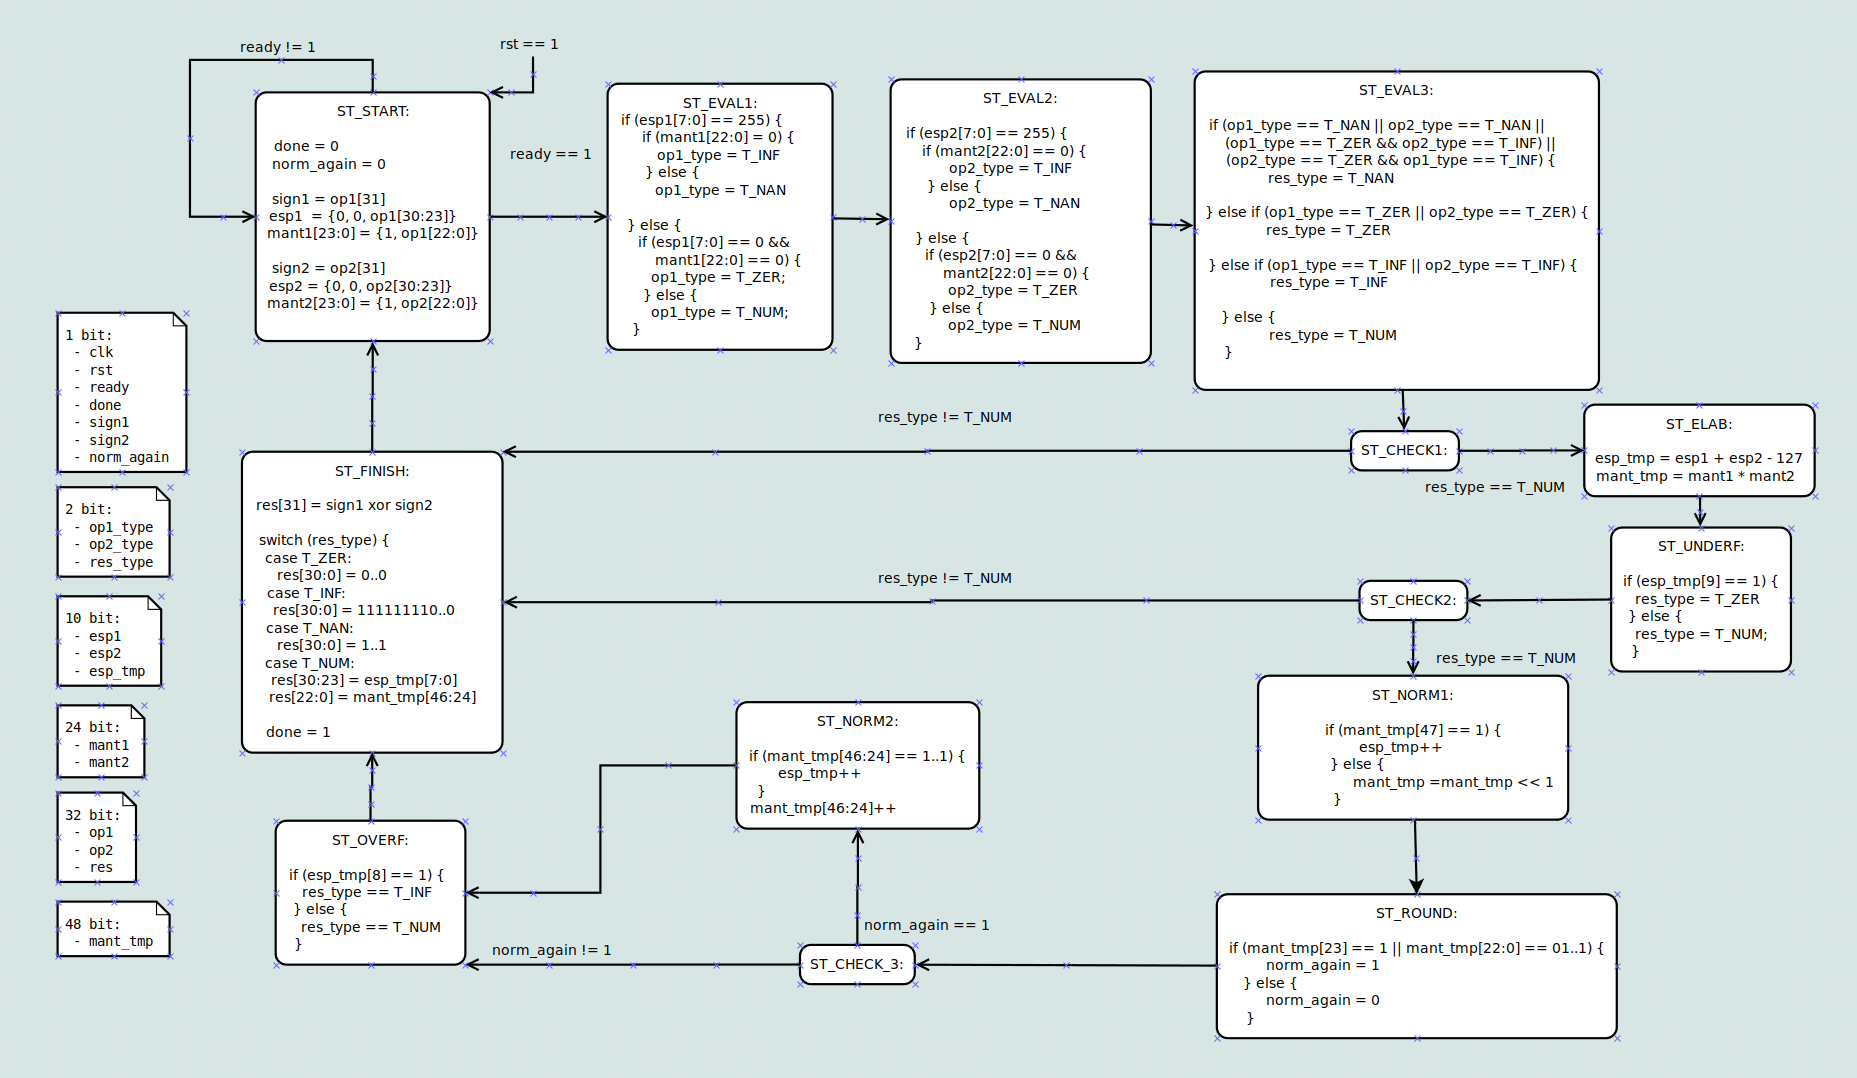
\includegraphics[width=\textwidth]{figures/EFSM-multiplier}
\caption{EFSM del multiplier}
\label{fig:EFSM1}
\end{figure*}

\begin{figure*}[bt]
\centering
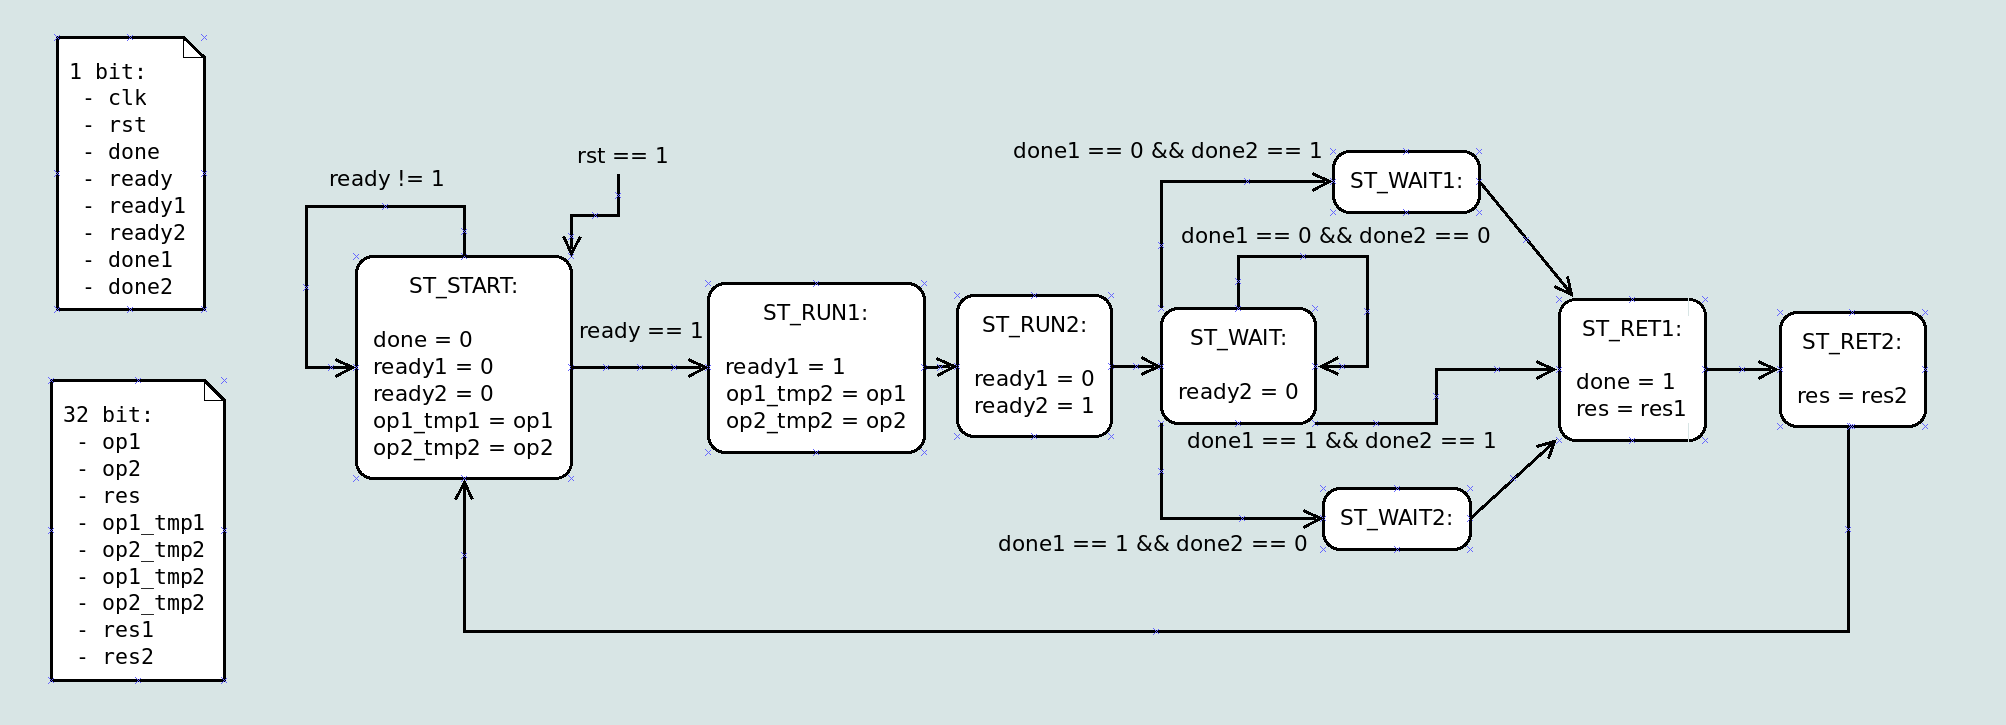
\includegraphics[width=\textwidth]{figures/EFSM-top_level}
\caption{EFSM del double\_multiplier}
\label{fig:EFSM2}
\end{figure*}

\begin{figure*}[bt]
\centering
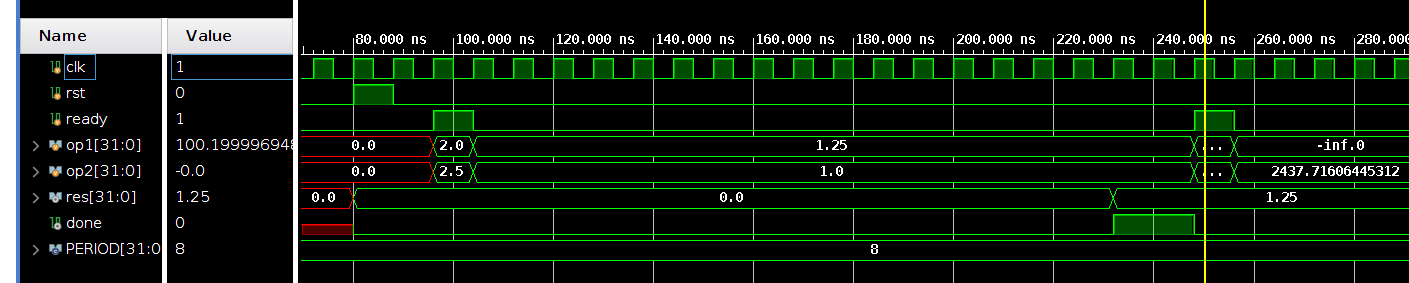
\includegraphics[width=\textwidth]{figures/simulazione1}
\caption{Simulazione in Verilog}
\label{fig:SIM1}
\end{figure*}

\begin{figure*}[bt]
\centering
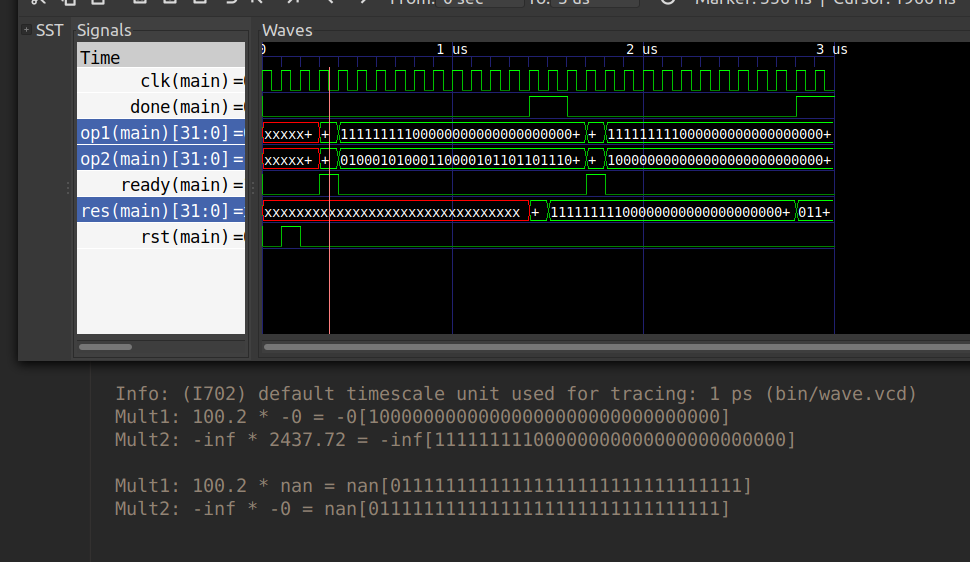
\includegraphics[width=\textwidth]{figures/simulazione2}
\caption{Simulazione in SystemC con targeted\_test}
\label{fig:SIM2}
\end{figure*}

\begin{figure*}[bt]
\centering
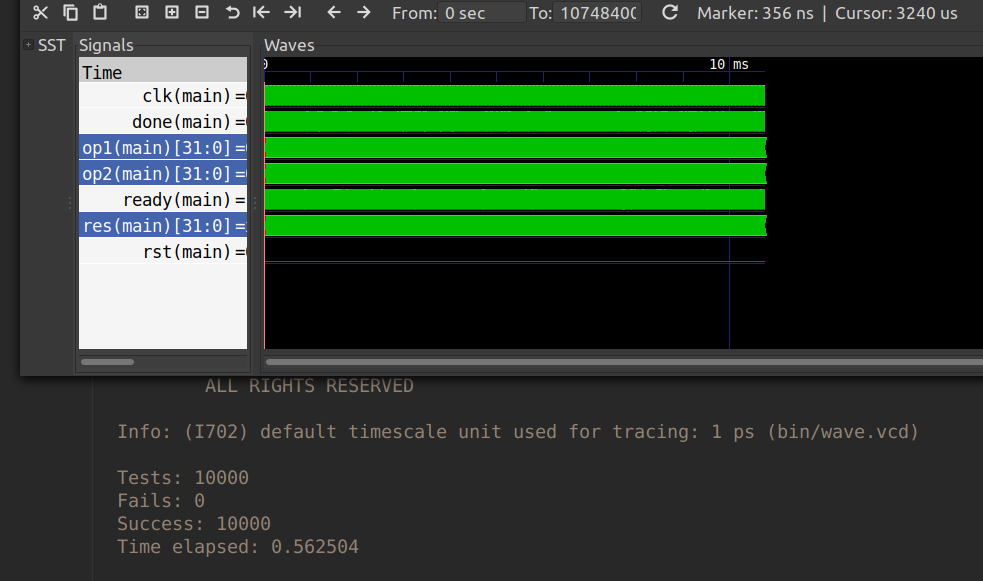
\includegraphics[width=\textwidth]{figures/simulazione3}
\caption{Simulazione in SystemC con rnd\_test}
\label{fig:SIM3}
\end{figure*}

\end{document}